\section{Неравенства решения}
1. $\cfrac{(x^2+5x-14)(x-3)^2}{|x+1|}\leqslant0\Leftrightarrow\cfrac{(x+7)(x-2)(x-3)^2}{|x+1|}\leqslant0.$ Применив метод интервалов, найдём ответ:
\begin{figure}[ht!]
\center{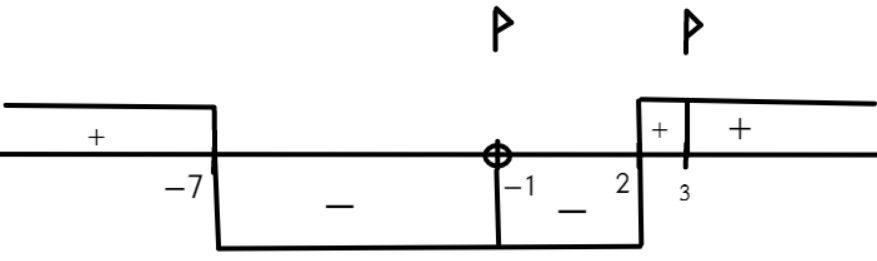
\includegraphics[scale=0.35]{int1.png}}
\end{figure}
$x\in[-7;-1)\cup(-1;2]\cup\{3\}.$\\
2. $\cfrac{(x^2-6x-16)(x+5)^2}{|x-2|}\leqslant0\Leftrightarrow\cfrac{(x-8)(x+2)(x+5)^2}{|x-2|}\leqslant0.$ Применив метод интервалов, найдём ответ:
\begin{figure}[ht!]
\center{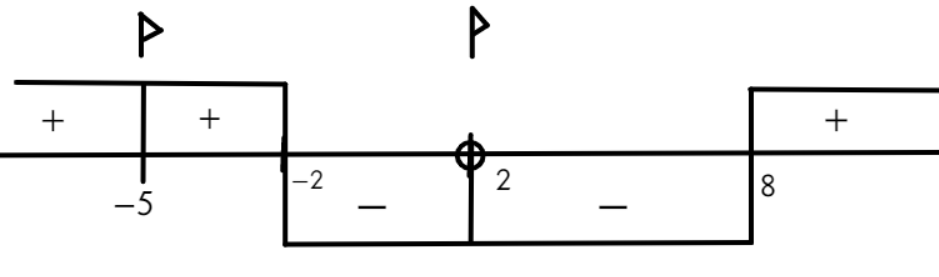
\includegraphics[scale=0.35]{int2.png}}
\end{figure}
$x\in\{-5\}\cup[-2;2)\cup(2;8].$\\
3. $\cfrac{(2x^2+7x-4)(x-3)^2}{x+6}\leqslant0\Leftrightarrow\cfrac{2\left(x-\cfrac{1}{2}\right)(x+4)(x-3)^2}{x+6}\leqslant0.$ Применив метод интервалов, найдём ответ:
\begin{figure}[ht!]
\center{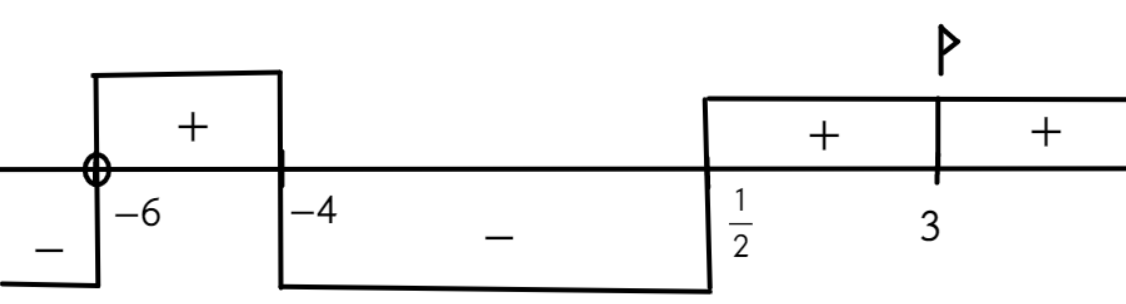
\includegraphics[scale=0.35]{int3.png}}
\end{figure}
$x\in(-\infty; -6)\cup\left[-4;\cfrac{1}{2}\right]\cup\{3\}.$\\
4. $\cfrac{(5x^2+6x+1)(x-2)^2}{x-4}\geqslant0\Leftrightarrow\cfrac{5\left(x+\cfrac{1}{5}\right)(x+1)(x-2)^2}{x-4}\geqslant0.$ Применив метод интервалов, найдём ответ:
\begin{figure}[ht!]
\center{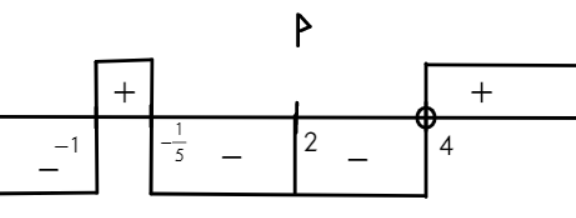
\includegraphics[scale=0.45]{int4.png}}
\end{figure}
$x\in\left[-1;-\cfrac{1}{5}\right]\cup\{2\}\cup(4;+\infty).$\newpage\noindent
5. $\cfrac{(x^2-1)(2x^2-5x-7)}{2-x}\leqslant0\Leftrightarrow\cfrac{(x-1)(x+1)^2\cdot 2\left(x-\cfrac{7}{2}\right)}{2-x}\leqslant0.$ Применив метод интервалов, найдём ответ:
\begin{figure}[ht!]
\center{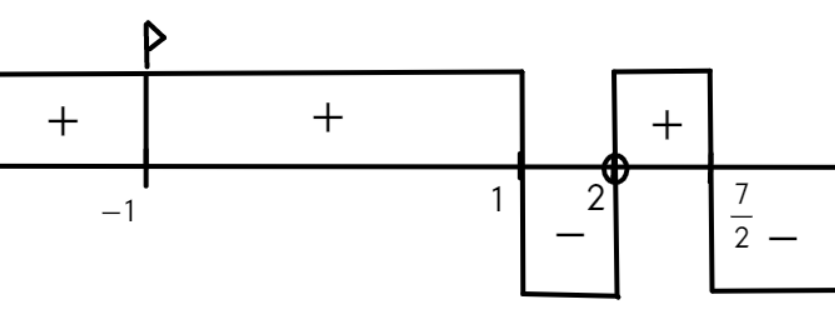
\includegraphics[scale=0.35]{int5.png}}
\end{figure}
$x\in\{-1\}\cup[1;2)\cup\left[\cfrac{7}{2};+\infty\right).$\\
6. $\cfrac{(x^2-1)(2x^2+5x-7)}{3-x}\leqslant0\Leftrightarrow\cfrac{(x-1)^2(x+1)\cdot 2\left(x+\cfrac{7}{2}\right)}{3-x}\leqslant0.$ Применив метод интервалов, найдём ответ:
\begin{figure}[ht!]
\center{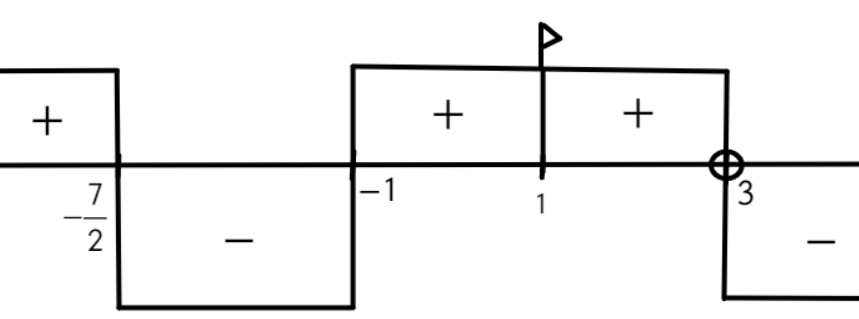
\includegraphics[scale=0.35]{int6.png}}
\end{figure}
$x\in\left[-\cfrac{7}{2};-1\right]\cup\{1\}\cup(3;+\infty).$\\
7. Сделаем замену: $x=\sqrt{a},\ y=\sqrt{b}.$ Тогда исходное неравенство примет вид $x^2+\cfrac{1}{x^2}+y^2+\cfrac{1}{y^2}\geqslant2xy+\cfrac{2}{xy}
\Leftrightarrow x^2-2xy+y^2+\cfrac{1}{x^2}-\cfrac{2}{xy}+\cfrac{1}{y^2}\geqslant0\Leftrightarrow (x-y)^2+\left(\cfrac{1}{x}-\cfrac{1}{y}\right)^2\geqslant0.$ Полученное неравенство верно для любых значений переменных, так как значения квадратов всегда неотрицательны.\\
8. Сделаем замену: $x=\sqrt{a},\ y=\sqrt{b},\ z=\sqrt{c}.$ Тогда исходное неравенство примет вид $x^2+y^2+z^2\geqslant xy+yz+xz\Leftrightarrow
2x^2+2y^2+2z^2\geqslant 2xy+2yz+2xz\Leftrightarrow x^2-2xy+y^2+y^2-2yz+z^2+x^2-2xz+z^2\geqslant 0\Leftrightarrow (x-y)^2+(y-z)^2+(x-z)^2\geqslant 0.$
Полученное неравенство верно для любых значений переменных, так как значения квадратов всегда неотрицательны.\\
9. Сделаем замену: $a=\sqrt{x},\ b=\sqrt{y}.$ Тогда требуется доказать неравенство $a^2-2b^2\leqslant 200$ при том, что $a-b=10.$ Выразим $a$ через $b$ и подставим:
$a=b+10,\ b^2+20b+100-2b^2\leqslant 200,\ b^2-20b+100\geqslant0,\ (b-10)^2\geqslant0.$ Полученное неравенство верно для любых значений переменных, так как значения квадратов всегда неотрицательны.\\
10. Сделаем замену: $a=\sqrt{x},\ b=\sqrt{y}.$ Тогда требуется доказать неравенство $a^2-2b^2\leqslant 128$ при том, что $a-b=8.$ Выразим $a$ через $b$ и подставим:
$a=b+8,\ b^2+16b+64-2b^2\leqslant 128,\ b^2-16b+64\geqslant0,\ (b-8)^2\geqslant0.$ Полученное неравенство верно для любых значений переменных, так как значения квадратов всегда неотрицательны.\\
11. $|2x+5|<x+4\Leftrightarrow\begin{cases}2x+5<x+4,\\ 2x+5>-x-4.\end{cases}
\Leftrightarrow\begin{cases}x<-1,\\ 3x>-9.\end{cases}\Leftrightarrow x\in (-3;-1).$\\
12. $|3x+7|<x+3\Leftrightarrow\begin{cases}3x+7<x+3,\\ 3x+7>-x-3.\end{cases}
\Leftrightarrow\begin{cases}2x<-4,\\ 4x>-10.\end{cases}\Leftrightarrow x\in \left(-\cfrac{5}{2};-2\right).$\newpage\noindent
13. $\sqrt{x}\cdot|1-x|\cdot(2-x)\cdot(3-x^2)\leqslant0 \Leftrightarrow \sqrt{x}\cdot|1-x|\cdot(x-2)\cdot(\sqrt{3}-x)\cdot(\sqrt{3}+x)\geqslant0.$
Применив метод интервалов, найдём ответ:
\begin{figure}[ht!]
\center{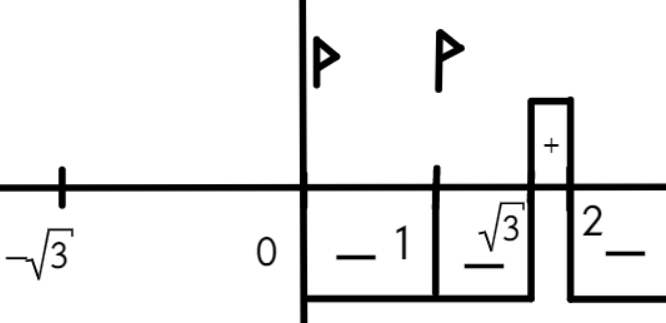
\includegraphics[scale=0.35]{int13.png}}
\end{figure}
$x\in\{0; 1\}\cup[\sqrt{3};2].$\\
14. $\sqrt{x}\cdot(1-x)\cdot|2-x|\cdot(3-x)^2\geqslant0.$
Применив метод интервалов, найдём ответ:
\begin{figure}[ht!]
\center{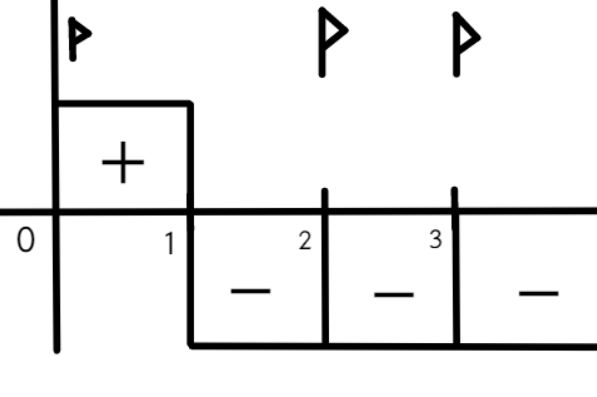
\includegraphics[scale=0.35]{int14.png}}
\end{figure}
$x\in[0;1]\cup\{2; 3\}.$\\
15. $|x+3|-|2x-4|<5\Leftrightarrow |x+3|<|2x-4|+5 \Leftrightarrow \left[\begin{array}{l}\begin{cases} -x-3<-2x+4+5,\\ x\leqslant -3.\end{cases}\\
\begin{cases} x+3<-2x+4+5,\\ -3\leqslant x\leqslant 2 .\end{cases}\\\begin{cases} x+3<2x-4+5,\\ 2\leqslant x.\end{cases}\end{array}\right.\Leftrightarrow
\left[\begin{array}{l}
x\in(-\infty;-3],\\
x\in[-3;2),\\
x\in(2;+\infty).\end{array}\right.\Leftrightarrow x\in(-\infty;2)\cup(2;+\infty)$\\
16. $|x-3|-|2x+4|<5\Leftrightarrow |x-3|<|2x+4|+5 \Leftrightarrow \left[\begin{array}{l}\begin{cases} -x+3<-2x-4+5,\\ x\leqslant -2.\end{cases}\\
\begin{cases} -x+3<2x+4+5,\\ -2\leqslant x\leqslant 3 .\end{cases}\\\begin{cases} -x+3<2x+4+5,\\ 3\leqslant x.\end{cases}\end{array}\right.\Leftrightarrow
\left[\begin{array}{l}
x\in(-\infty;-2),\\
x\in(-2;3],\\
x\in[3;+\infty).\end{array}\right.\Leftrightarrow x\in(-\infty;-2)\cup(-2;+\infty)$\\
17. $\cfrac{x^2+3}{x+1}\leqslant2\Leftrightarrow \cfrac{x^2+3-2x-2}{x+1}\leqslant0\Leftrightarrow \cfrac{(x-1)^2}{x+1}\leqslant0\Leftrightarrow
\left[\begin{array}{l}
x-1=0,\\
x+1<0
\end{array}\right.\Leftrightarrow x \in (-\infty;-1)\cup\{1\}.$\\
18. $\cfrac{x^2}{x-1}\leqslant 4 \Leftrightarrow \cfrac{x^2-4x+4}{x-1}\leqslant 0 \Leftrightarrow \cfrac{(x-2)^2}{x-1}\leqslant 0
\Leftrightarrow
\left[\begin{array}{l}
x-2=0,\\
x-1<0
\end{array}\right.\Leftrightarrow x \in (-\infty;1)\cup\{2\}.$\\
19. $|3x-7|+|x+2|>7\Leftrightarrow \left[\begin{array}{l}\begin{cases} -3x+7-x-2>7,\\ x\leqslant -2.\end{cases}\\
\begin{cases} -3x+7+x+2>7,\\ -2\leqslant x\leqslant \cfrac{7}{3}.\end{cases}\\\begin{cases} 3x-7+x+2>7,\\ \cfrac{7}{3}\leqslant x.\end{cases}\end{array}\right.\Leftrightarrow
\left[\begin{array}{l}
x\in(-\infty;-2],\\
x\in[-2;1),\\
x\in(3;+\infty).\end{array}\right.\Leftrightarrow x\in(-\infty;1)\cup(3;+\infty)$\newpage\noindent
20. $\cfrac{\sqrt{x-3}}{(x-1)(x-5)^2(x-6)}\leqslant0.$
Применив метод интервалов, найдём ответ:
\begin{figure}[ht!]
\center{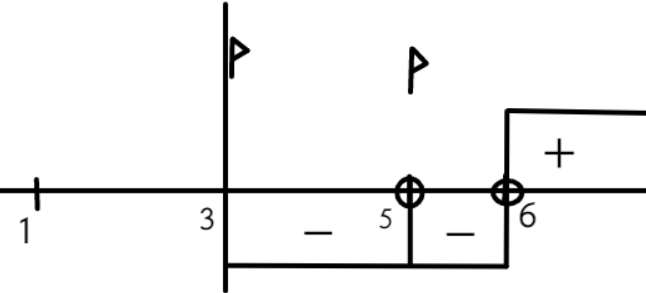
\includegraphics[scale=0.35]{int20.png}}
\end{figure}
$x\in[3;5)\cup(5;6).$\\
21. $\cfrac{\sqrt{x-4}}{(x-2)(x-6)^2(x-7)}\leqslant0.$
Применив метод интервалов, найдём ответ:
\begin{figure}[ht!]
\center{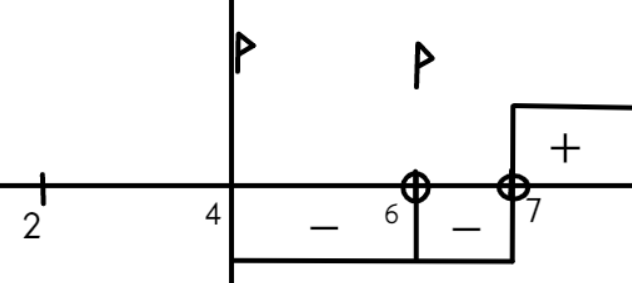
\includegraphics[scale=0.35]{int21.png}}
\end{figure}
$x\in[4;6)\cup(6;7).$\\
22. $|x|\cdot\cfrac{x^3+x^2-x-1}{x^3-x^2-x+1}\geqslant 0\Leftrightarrow|x|\cdot\cfrac{x^2(x+1)-(x+1)}{x^2(x-1)-(x-1)}\geqslant 0\Leftrightarrow
|x|\cdot\cfrac{(x-1)(x+1)^2}{(x-1)^2(x+1)}\geqslant 0.$
Применив метод интервалов, найдём ответ:
\begin{figure}[ht!]
\center{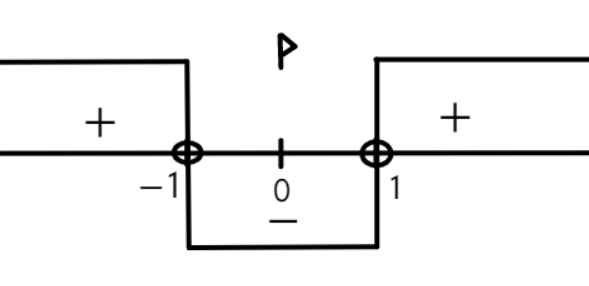
\includegraphics[scale=0.35]{int22.png}}
\end{figure}
$x\in(-\infty;-1)\cup\{0\}\cup(1;+\infty).$\\
23. $|x|\cdot\cfrac{x^3-x^2-x+1}{x^3+x^2-x-1}\geqslant 0\Leftrightarrow|x|\cdot\cfrac{x^2(x-1)-(x-1)}{x^2(x+1)-(x+1)}\geqslant 0\Leftrightarrow
|x|\cdot\cfrac{(x-1)^2(x+1)}{(x-1)(x+1)^2}\geqslant 0.$
Применив метод интервалов, найдём ответ:
\begin{figure}[ht!]
\center{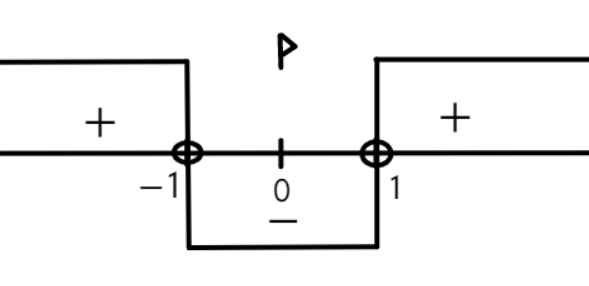
\includegraphics[scale=0.35]{int22.png}}
\end{figure}
$x\in(-\infty;-1)\cup\{0\}\cup(1;+\infty).$\\
24. $|2x-3|<4+x\Leftrightarrow\begin{cases}2x-3<4+x,\\ 2x-3>-4-x.\end{cases}
\Leftrightarrow\begin{cases}x<7,\\ 3x>-1.\end{cases}\Leftrightarrow
x\in\left(-\cfrac{1}{3};7\right).$\\
25. $|2x-1|<5+x\Leftrightarrow\begin{cases}2x-1<5+x,\\ 2x-1>-5-x.\end{cases}
\Leftrightarrow\begin{cases}x<6,\\ 3x>-4.\end{cases}\Leftrightarrow x\in \left(-\cfrac{4}{3};6\right).$\\
26. $\cfrac{(x-1)^2(x+3)(x-3)}{\sqrt{x+2}}\geqslant0.$ Применив метод интервалов, найдём ответ:
\begin{figure}[ht!]
\center{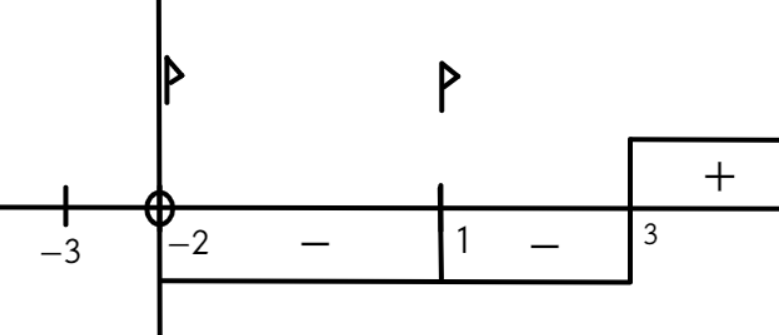
\includegraphics[scale=0.35]{int26.png}}
\end{figure}
$x\in\{1\}\cup[3;+\infty).$\newpage\noindent
27. $\cfrac{(x-2)^2(x+2)(x-4)}{\sqrt{x+1}}\geqslant0.$
Применив метод интервалов, найдём ответ:
\begin{figure}[ht!]
\center{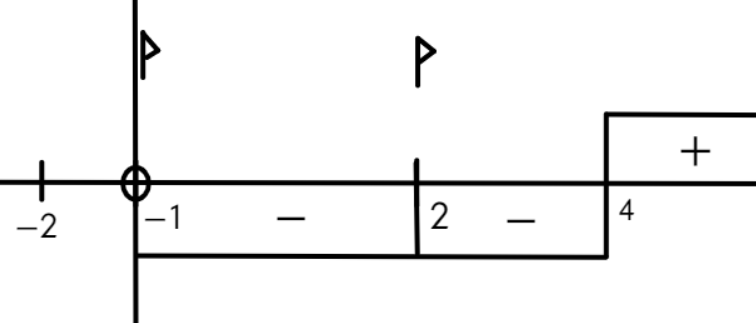
\includegraphics[scale=0.35]{int27.png}}
\end{figure}
$x\in\{2\}\cup[4;+\infty).$\\
28. $\cfrac{x^2-3}{x+2}\geqslant-6\Leftrightarrow \cfrac{x^2-3+6x+12}{x+2}\geqslant0\Leftrightarrow \cfrac{(x+3)^2}{x+2}\geqslant0
\Leftrightarrow
\left[\begin{array}{l}
x+3=0,\\
x+2>0
\end{array}\right.\Leftrightarrow x \in \{-3\}\cup(-2;+\infty).$\\
29. $\cfrac{x^2-3}{x-2}\leqslant 6\Leftrightarrow \cfrac{x^2-3-6x+12}{x-2}\leqslant0\Leftrightarrow \cfrac{(x-3)^2}{x-2}\leqslant0
\Leftrightarrow
\left[\begin{array}{l}
x-3=0,\\
x-2<0
\end{array}\right.\Leftrightarrow x \in (-\infty;2)\cup\{3\}.$\\
30. $\cfrac{(x-1)^2(x^2-x-2)}{x^2+3x+2}\geqslant0\Leftrightarrow\cfrac{(x-1)^2(x-2)(x+1)}{(x+2)(x+1)}\geqslant0.$
Применив метод интервалов, найдём ответ:
\begin{figure}[ht!]
\center{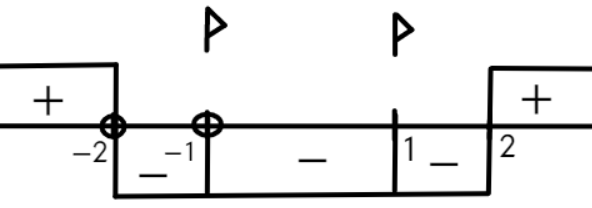
\includegraphics[scale=0.35]{int30.png}}
\end{figure}
$x\in(-\infty;-2)\cup\{1\}\cup[2;+\infty).$\\
31. $\cfrac{(x+1)^2(x^2+x-2)}{x^2-3x+2}\geqslant0\Leftrightarrow\cfrac{(x+1)^2(x+2)(x-1)}{(x-2)(x-1)}\geqslant0.$
Применив метод интервалов, найдём ответ:
\begin{figure}[ht!]
\center{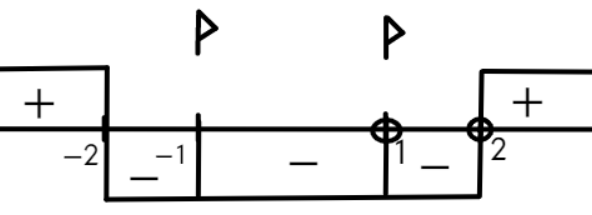
\includegraphics[scale=0.35]{int31.png}}
\end{figure}
$x\in(-\infty;-2]\cup\{-1\}\cup(2;+\infty).$\\
32. $\cfrac{x^2}{x+2}\leqslant -x\Leftrightarrow\cfrac{x^2+x^2+2x}{x+2}\leqslant 0\Leftrightarrow\cfrac{2x(x+1)}{x+2}\leqslant 0.$
Применив метод интервалов, найдём ответ:
\begin{figure}[ht!]
\center{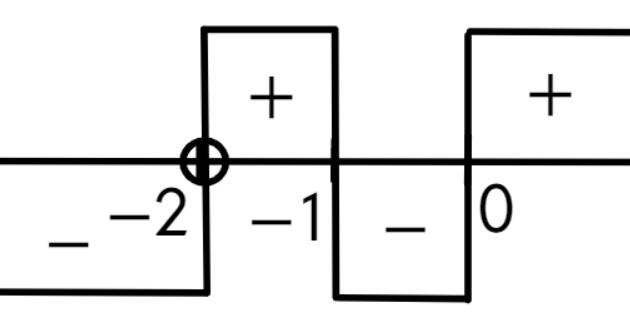
\includegraphics[scale=0.35]{int32.png}}
\end{figure}
$x\in(-\infty;-2)\cup[-1;0].$\\
33. $\cfrac{x^2}{2-x}\leqslant x \Leftrightarrow\cfrac{x^2-2x+x^2}{2-x}\leqslant 0\Leftrightarrow\cfrac{2x(x-1)}{2-x}\leqslant 0.$
Применив метод интервалов, найдём ответ:
\begin{figure}[ht!]
\center{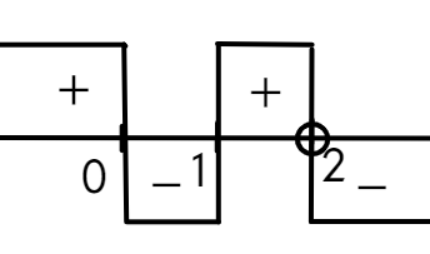
\includegraphics[scale=0.35]{int33.png}}
\end{figure}
$x\in[0;1]\cup(2;+\infty).$\\
34. $|3x+2|\geqslant x^2-2\Leftrightarrow\left[\begin{array}{l}3x+2\geqslant x^2-2,\\ 3x+2\leqslant -x^2+2.\end{array}\right.\Leftrightarrow
\left[\begin{array}{l}x^2-3x-4\leqslant 0,\\ x^2+3x\leqslant 0.\end{array}\right.\Leftrightarrow
\left[\begin{array}{l}(x-4)(x+1)\leqslant 0,\\ x(x+3)\leqslant 0.\end{array}\right.
\Leftrightarrow
\left[\begin{array}{l}x\in[-1;4],\\ x\in[-3;0].\end{array}\right.\Leftrightarrow
x\in[-3;4].$\\
35. $|2-3x|\geqslant x^2-2\Leftrightarrow\left[\begin{array}{l}2-3x\geqslant x^2-2,\\ 2-3x\leqslant -x^2+2.\end{array}\right.\Leftrightarrow
\left[\begin{array}{l}x^2+3x-4\leqslant 0,\\ x^2-3x\leqslant 0.\end{array}\right.\Leftrightarrow
\left[\begin{array}{l}(x+4)(x-1)\leqslant 0,\\ x(x-3)\leqslant 0.\end{array}\right.
\Leftrightarrow
\left[\begin{array}{l}x\in[-4;1],\\ x\in[0;3].\end{array}\right.\Leftrightarrow
x\in[-4;3].$\\
36. $\cfrac{3}{x}<5\Leftrightarrow \cfrac{5\left(\cfrac{3}{5}-x\right)}{x}<0\Leftrightarrow x\in(-\infty;0)\cup\left(\cfrac{3}{5};+\infty\right).$\\
37. $\cfrac{7}{x}<4\Leftrightarrow \cfrac{4\left(\cfrac{7}{4}-x\right)}{x}<0\Leftrightarrow x\in(-\infty;0)\cup\left(\cfrac{7}{4};+\infty\right).$\\
38. $x^2-3x+2>|x-5|\Leftrightarrow \begin{cases}x-5<x^2-3x+2,\\ x-5>-x^2+3x-2.\end{cases}
\Leftrightarrow \begin{cases}x^2-4x+7>0,\\ x^2-2x-3>0.\end{cases}
\Leftrightarrow \begin{cases}(x-2)^2+3>0,\\ (x-3)(x+1)>0.\end{cases}$\\$\Leftrightarrow x\in (-\infty;-1)\cup(3;+\infty).$\\
39. $x^2-5x+6>|x-6|\Leftrightarrow \begin{cases}x-6<x^2-5x+6,\\ x-6>-x^2+5x-6.\end{cases}
\Leftrightarrow \begin{cases}x^2-6x+12>0,\\ x^2-4x>0.\end{cases}
\Leftrightarrow \begin{cases}(x-3)^2+3>0,\\ x(x-4)>0.\end{cases}$\\$\Leftrightarrow x\in (-\infty;0)\cup(4;+\infty).$\\
40. $\cfrac{1}{x-2}+\cfrac{1}{x-1}\geqslant\cfrac{1}{x}\Leftrightarrow \cfrac{x(x-1)+x(x-2)-(x-1)(x-2)}{x(x-1)(x-2)}\geqslant0\Leftrightarrow$\\$
\cfrac{x^2-x+x^2-2x-x^2+2x+x-2}{x(x-1)(x-2)}\geqslant0\Leftrightarrow\cfrac{(x-\sqrt{2})(x+\sqrt{2})}{x(x-1)(x-2)}\geqslant0.$\\ Применив метод интервалов, найдём ответ:
\begin{figure}[ht!]
\center{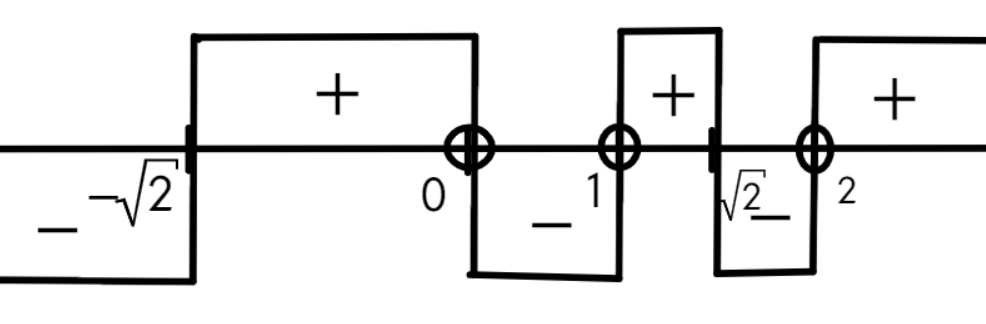
\includegraphics[scale=0.35]{int40.png}}
\end{figure}
$x\in[-\sqrt{2};0)\cup(1;\sqrt{2}]\cup(2;+\infty).$\\
41. $\cfrac{1}{x+2}+\cfrac{1}{x+1}\geqslant\cfrac{1}{x}\Leftrightarrow \cfrac{x(x+1)+x(x+2)-(x+1)(x+2)}{x(x+1)(x+2)}\geqslant0\Leftrightarrow$\\$
\cfrac{x^2+x+x^2+2x-x^2-2x-x-2}{x(x+1)(x+2)}\geqslant0\Leftrightarrow\cfrac{(x-\sqrt{2})(x+\sqrt{2})}{x(x+1)(x+2)}\geqslant0.$\\ Применив метод интервалов, найдём ответ:
\begin{figure}[ht!]
\center{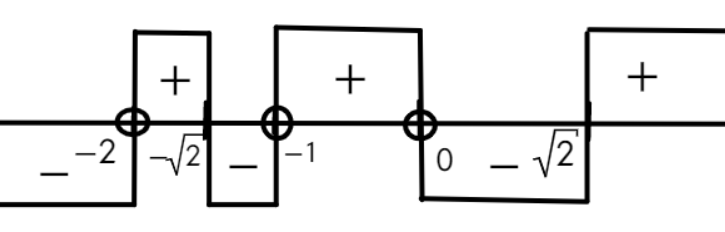
\includegraphics[scale=0.35]{int41.png}}
\end{figure}
$x\in(-2;-\sqrt{2}]\cup(-1;0)\cup[\sqrt{2};+\infty).$\newpage\noindent
42. $\cfrac{1}{x-2}+\cfrac{1}{x-3}\geqslant\cfrac{1}{x}\Leftrightarrow \cfrac{x(x-3)+x(x-2)-(x-3)(x-2)}{x(x-2)(x-3)}\geqslant0\Leftrightarrow$\\$
\cfrac{x^2-3x+x^2-2x-x^2+2x+3x-6}{x(x-2)(x-3)}\geqslant0\Leftrightarrow\cfrac{(x-\sqrt{6})(x+\sqrt{6})}{x(x-2)(x-3)}\geqslant0.$\\ Применив метод интервалов, найдём ответ:
\begin{figure}[ht!]
\center{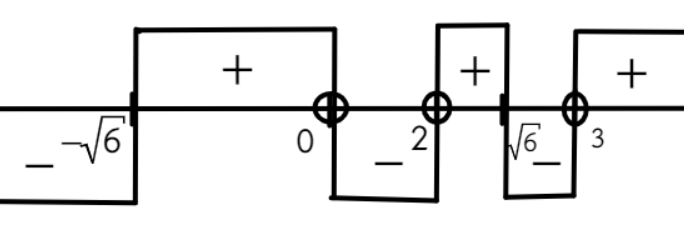
\includegraphics[scale=0.35]{int42.png}}
\end{figure}
$x\in[-\sqrt{6};0)\cup(2;\sqrt{6}]\cup(3;+\infty).$\\
43. $\cfrac{1}{x+2}+\cfrac{1}{x+3}\geqslant\cfrac{1}{x}\Leftrightarrow \cfrac{x(x+3)+x(x+2)-(x+3)(x+2)}{x(x+2)(x+3)}\geqslant0\Leftrightarrow$\\$
\cfrac{x^2+3x+x^2+2x-x^2-2x-3x-6}{x(x+2)(x+3)}\geqslant0\Leftrightarrow\cfrac{(x-\sqrt{6})(x+\sqrt{6})}{x(x+2)(x+3)}\geqslant0.$\\ Применив метод интервалов, найдём ответ:
\begin{figure}[ht!]
\center{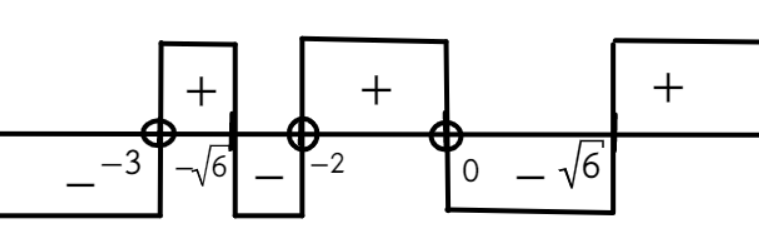
\includegraphics[scale=0.35]{int43.png}}
\end{figure}
$x\in(-3;-\sqrt{6}]\cup(-2;0)\cup[\sqrt{6};+\infty).$\\
44. $|x^2-6x-7|\geqslant-6x+7\Leftrightarrow \left[\begin{array}{l}x^2-6x-7\geqslant -6x+7,\\ x^2-6x-7\leqslant 6x-7.\end{array}\right.
\Leftrightarrow \left[\begin{array}{l}(x-\sqrt{14})(x+\sqrt{14})\geqslant 0,\\ x(x-12)\leqslant 0.\end{array}\right.
\Leftrightarrow$\\$ \left[\begin{array}{l}x\in(-\infty;-\sqrt{14}]\cup[\sqrt{14};+\infty),\\ x\in[0;12].\end{array}\right.\Leftrightarrow
x\in(-\infty;-\sqrt{14}]\cup[0;+\infty).$\\
45. $|x^2-2x-15|\leqslant-2x+15\Leftrightarrow \begin{cases}x^2-2x-15\leqslant -2x+15,\\ x^2-2x-15\geqslant 2x-15.\end{cases}
\Leftrightarrow \begin{cases}(x-\sqrt{30})(x+\sqrt{30})\leqslant 0,\\ x(x-4)\geqslant 0.\end{cases}
\Leftrightarrow$\\$ \begin{cases} x\in[-\sqrt{30};\sqrt{30}],\\ x\in(-\infty;0]\cup[4;+\infty).\end{cases}\Leftrightarrow
x\in[-\sqrt{30};0]\cup[4;\sqrt{30}].$\\
46. $\cfrac{x^2-2x-8}{x-4}\leqslant 7\Leftrightarrow \cfrac{x^2-2x-8-7x+28}{x-4}\leqslant0 \Leftrightarrow \cfrac{(x-5)(x-4)}{x-4}\leqslant0
\Leftrightarrow \begin{cases}x-5\leqslant 0,\\ x-4\neq0.\end{cases}\Leftrightarrow$\\$ x\in (-\infty;4)\cup(4;5].$\\
47. $\cfrac{x^2-4x-5}{x-5}\leqslant 7\Leftrightarrow \cfrac{x^2-4x-5-7x+35}{x-5}\leqslant0 \Leftrightarrow \cfrac{(x-5)(x-6)}{x-5}\leqslant0
\Leftrightarrow \begin{cases}x-6\leqslant 0,\\ x-5\neq0.\end{cases}\Leftrightarrow$\\$ x\in (-\infty;5)\cup(5;6].$\\
48. $\cfrac{7}{(x-1)(x-2)}+\cfrac{9}{x-2}+1\leqslant0\Leftrightarrow \cfrac{7+9x-9+x^2-2x-x+2}{(x-1)(x-2)}\leqslant0
\Leftrightarrow \cfrac{x(x+6)}{(x-1)(x-2)}\leqslant0.$ Применив метод интервалов, найдём ответ:
\begin{figure}[ht!]
\center{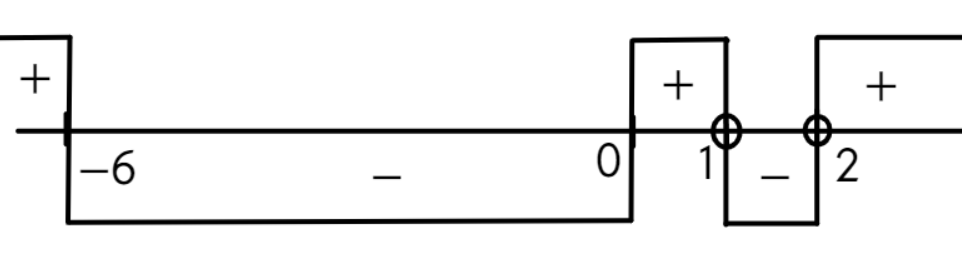
\includegraphics[scale=0.35]{int48.png}}
\end{figure}
$x\in[-6;0]\cup(1;2).$\newpage\noindent
49. $\cfrac{1}{3-x}\geqslant\cfrac{1}{(x^2-9)(3-x)}\Leftrightarrow\cfrac{-1}{(x-3)^2(x+3)}-\cfrac{1}{3-x}\leqslant0\Leftrightarrow
\cfrac{-1+x^2-9}{(x-3)^2(x+3)}\leqslant0\Leftrightarrow$\\$\cfrac{(x-\sqrt{10})(x+\sqrt{10})}{(x-3)^2(x+3)}\leqslant0.$\\ Применив метод интервалов, найдём ответ:
\begin{figure}[ht!]
\center{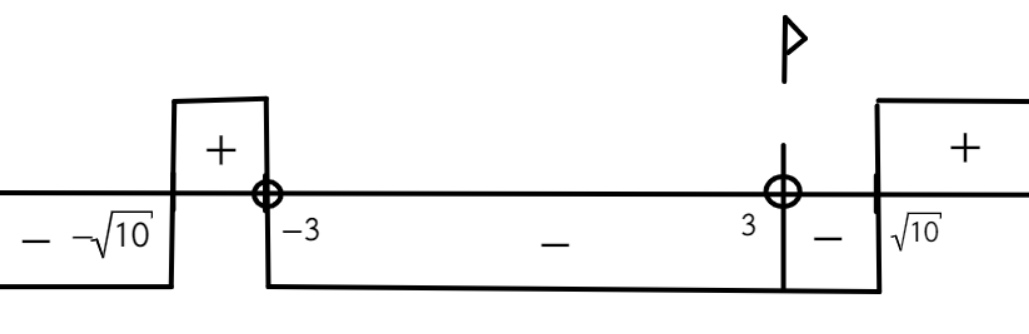
\includegraphics[scale=0.35]{int49.png}}
\end{figure}
$x\in(-\infty;-\sqrt{10}]\cup(-3;3)\cup(3;\sqrt{10}].$\\
50. $\cfrac{1}{(4-x^2)(x-2)}\leqslant\cfrac{1}{2-x} \Leftrightarrow\cfrac{-1}{(x-2)^2(x+2)}-\cfrac{1}{2-x}\leqslant0\Leftrightarrow
\cfrac{-1+x^2-4}{(x-2)^2(x+2)}\leqslant0\Leftrightarrow$\\$\cfrac{(x-\sqrt{5})(x+\sqrt{5})}{(x-2)^2(x+2)}\leqslant0.$\\ Применив метод интервалов, найдём ответ:
\begin{figure}[ht!]
\center{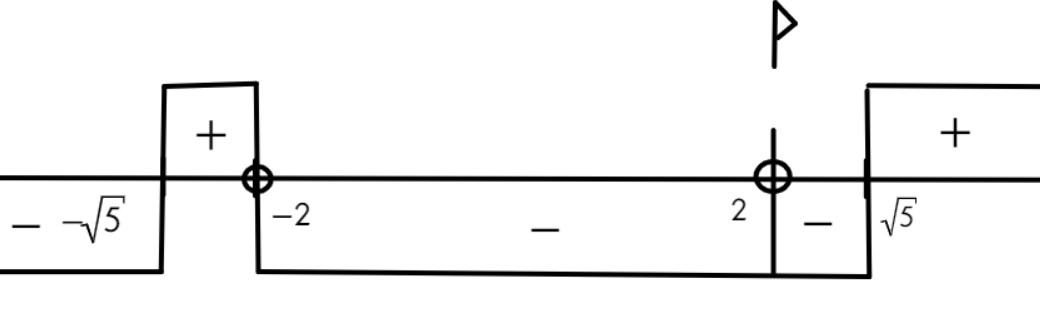
\includegraphics[scale=0.35]{int50.png}}
\end{figure}
$x\in(-\infty;-\sqrt{5}]\cup(-2;2)\cup(2;\sqrt{5}].$\\
51. $\cfrac{x^2-(\sqrt{3}+\sqrt{7})x+\sqrt{21}}{\sqrt{5-x}}\cdot\cfrac{x^2-4x+4}{6x-x^2-9}\leqslant 0\Leftrightarrow
\cfrac{(x-\sqrt{3})(x-\sqrt{7})(x-2)^2}{\sqrt{5-x}(x-3)^2}\geqslant 0.$ Применив метод интервалов, найдём ответ:
\begin{figure}[ht!]
\center{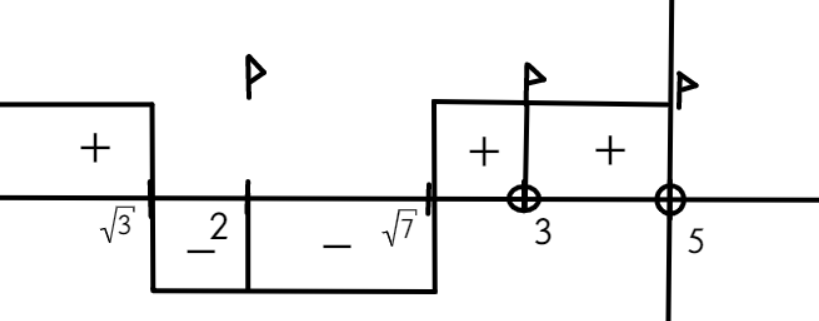
\includegraphics[scale=0.35]{int51.png}}
\end{figure}
$x\in(-\infty;\sqrt{3}]\cup\{2\}\cup[\sqrt{7};3)\cup(3;5).$\\
52. $\cfrac{\sqrt{x}}{2x-1}\geqslant\cfrac{\sqrt{x}}{x-5}\Leftrightarrow\sqrt{x}\cdot\left(\cfrac{1}{2x-1}-\cfrac{1}{x-5}\right)\geqslant0\Leftrightarrow
\cfrac{\sqrt{x}(-4-x)}{(2x-1)(x-5)}\geqslant0.$ Применив метод интервалов, найдём ответ:
\begin{figure}[ht!]
\center{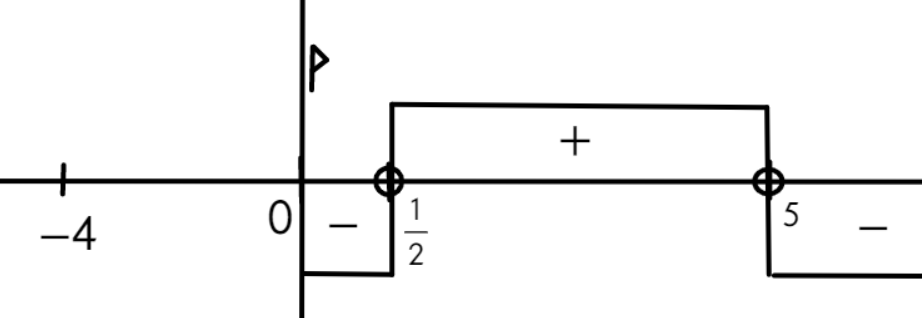
\includegraphics[scale=0.35]{int52.png}}
\end{figure}
$x\in\{0\}\cup\left(\cfrac{1}{2};5\right).$\\
53. $x\sqrt{x+2}>x\Leftrightarrow x(\sqrt{x+2}-1)>0.$ Это неравенство также можно решить методом интервалов, поставив на числовом луче две точки 0 и $-1$ (так как второй множитель равен нулю при  $x=-1).$ По ОДЗ значение $x$ не может быть меньше $-2,$ поэтому получим ответ $x\in[-2;-1)\cup(0;+\infty).$\newpage\noindent
54. $\cfrac{3x^2+2x^3-x^4}{\sqrt{x+2}}\leqslant0\Leftrightarrow\cfrac{x^2(3+2x-x^2)}{\sqrt{x+2}}\leqslant0
\Leftrightarrow\cfrac{x^2(x-3)(x+1)}{\sqrt{x+2}}\geqslant0.$ Применив метод интервалов, найдём ответ:
\begin{figure}[ht!]
\center{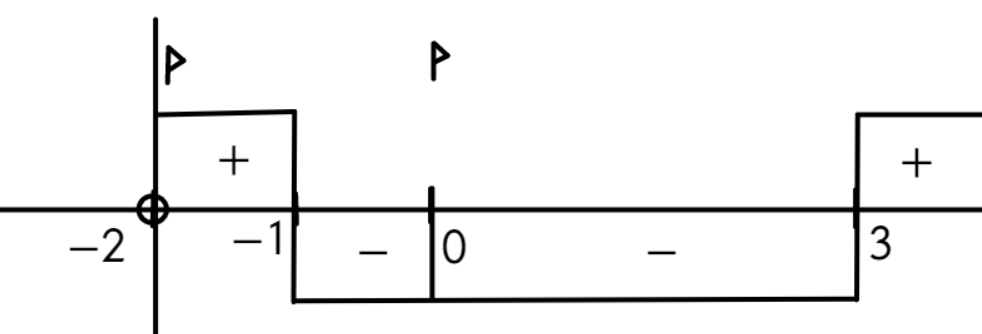
\includegraphics[scale=0.35]{int54.png}}
\end{figure}
$x\in(-2;-1]\cup\{0\}\cup[3;+\infty).$\\
55. $x|x-2|\leqslant x-2\Leftrightarrow \left[\begin{array}{l}x-2=0,\\ x \leqslant \cfrac{x-2}{|x-2|}.\end{array}\right.
\Leftrightarrow \left[\begin{array}{l}x=2,\\ \begin{cases}x \leqslant 1,\\ x>2.\end{cases}\\ \begin{cases}x \leqslant -1,\\ x<2.\end{cases} \end{array}\right.
\Leftrightarrow x\in (-\infty;-1]\cup\{2\}.$\\
56. $-\cfrac{1}{2}x^2+2,5x-3\geqslant0\Leftrightarrow x^2-5x+6\leqslant0\Leftrightarrow (x-2)(x-3)\leqslant0\Leftrightarrow
x\in[2;3].$\\
57. $\cfrac{4}{x^2-x-6}\geqslant\cfrac{1}{2+x}\Leftrightarrow\cfrac{4}{(x-3)(x+2)}-\cfrac{1}{x+2}\geqslant0\Leftrightarrow
\cfrac{7-x}{(x-3)(x+2)}\geqslant0.$ Применив метод интервалов, найдём ответ:
\begin{figure}[ht!]
\center{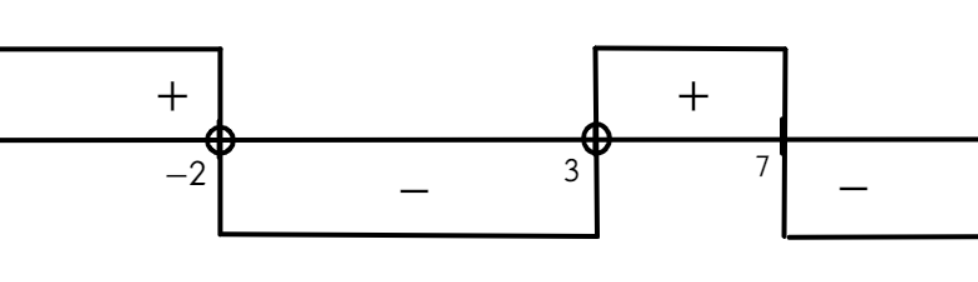
\includegraphics[scale=0.35]{int57.png}}
\end{figure}
$x\in(-\infty;-2)\cup(3;7].$\\
58. $x^2-x>|x+3|\Leftrightarrow \begin{cases}x+3<x^2-x,\\ x+3>-x^2+x.\end{cases}\Leftrightarrow \begin{cases}x^2-2x-3>0,\\ x^2+3>0.\end{cases}\Leftrightarrow
(x-3)(x+1)>0\Leftrightarrow $\\$x\in(-\infty;-1)\cup(3;+\infty).$\\
59. $|x^2-3|<|3-x|\Leftrightarrow (x^2-3+3-x)(x^2-3-3+x)<0 \Leftrightarrow x(x-1)(x+3)(x-2)<0.$ Применив метод интервалов, найдём ответ:
\begin{figure}[ht!]
\center{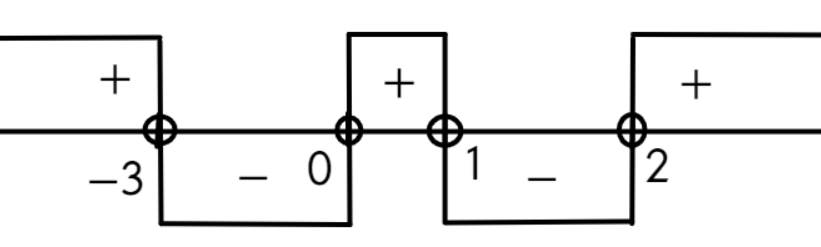
\includegraphics[scale=0.35]{int59.png}}
\end{figure}
$x\in(-3;0)\cup(1;2).$\\
60. $\cfrac{x^2-20}{5x^2+12}\leqslant\cfrac{x-8}{5x^2+12}\Leftrightarrow\cfrac{x^2-20-x+8}{5x^2+12}\leqslant0\Leftrightarrow
\cfrac{(x-4)(x+3)}{5x^2+12}\leqslant0\Leftrightarrow x\in [-3;4].$\\
61. $\left(1+\left(x-\cfrac{3}{2}\right):3\right)\left(-0,75\right)<0\Leftrightarrow1+\left(x-\cfrac{3}{2}\right):3>0\Leftrightarrow
x-\cfrac{3}{2}>-3\Leftrightarrow x\in  \left(-\cfrac{3}{2};+\infty\right).$\\
62. $x^2+x>|x-3|\Leftrightarrow \begin{cases}x-3<x^2+x,\\ x-3>-x^2-x.\end{cases}\Leftrightarrow \begin{cases}x^2+3>0,\\ x^2+2x-3>0.\end{cases}\Leftrightarrow
(x+3)(x-1)>0\Leftrightarrow $\\$x\in(-\infty;-3)\cup(1;+\infty).$\\
63. Если $x<6,$ то по крайней мере первое из чисел меньше 6, а значит меньшее из двух чисел точно меньше 6. Если же $x\geqslant6,$ то и $x^2-3\geqslant36-3=33>6.$ Таким образом, подходят только значения $x<6.$\\
64. Чтобы минимальное из двух чисел было не меньше 4, необходимо и достаточно, чтобы они оба были не меньше 4. То есть, надо решить систему неравенств\\
$\begin{cases}x+15 \geqslant 4,\\ x^2+3\geqslant 4.\end{cases}\Leftrightarrow
\begin{cases}x \geqslant -11,\\(x-1)(x+1)\geqslant 0.\end{cases}\Leftrightarrow
\begin{cases}x \geqslant -11,\\ x\in(-\infty;-1]\cup[1;+\infty).\end{cases}\Leftrightarrow
x \in [-11;-1]\cup[1;+\infty).$\\
65. Чтобы максимальное из двух чисел было не меньше 1, необходимо и достаточно, чтобы хотя бы одно из них было не меньше 1. То есть, надо решить совокупность неравенств\\ $\left[\begin{array}{l}x\geqslant 1,\\ x^2-3 \geqslant1 .  \end{array}\right.\Leftrightarrow
\left[\begin{array}{l}x\geqslant 1,\\ (x-2)(x+2) \geqslant 0 .  \end{array}\right.\Leftrightarrow
\left[\begin{array}{l}x\geqslant 1,\\ x\in (-\infty;-2]\cup[2;+\infty).  \end{array}\right.\Leftrightarrow
x\in (-\infty;-2]\cup[1;+\infty).$\\
66. $\cfrac{2x^3+3x^2}{x-2}\geqslant0\Leftrightarrow\cfrac{2x^2\left(x+\cfrac{3}{2}\right)}{x-2}\geqslant0.$\\ Применив метод интервалов, найдём ответ:
\begin{figure}[ht!]
\center{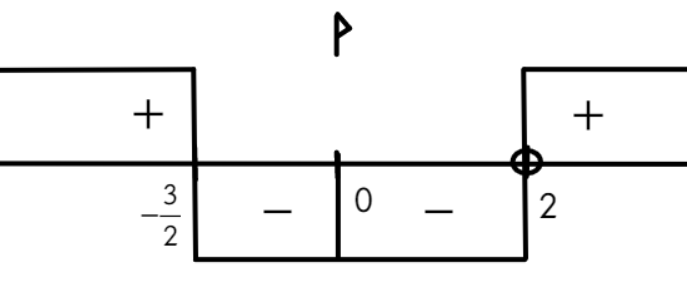
\includegraphics[scale=0.35]{int66.png}}
\end{figure}
$x\in\left(-\infty;-\cfrac{3}{2}\right]\cup\{0\}\cup(2;+\infty).$\\
67. $\cfrac{2x^3-3x^2}{x+2}\geqslant0\Leftrightarrow\cfrac{2x^2\left(x-\cfrac{3}{2}\right)}{x+2}\geqslant0.$\\ Применив метод интервалов, найдём ответ:
\begin{figure}[ht!]
\center{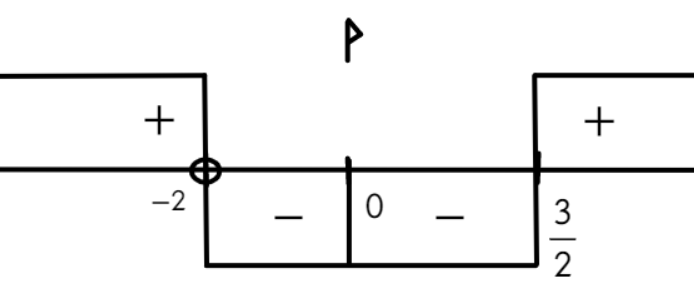
\includegraphics[scale=0.35]{int67.png}}
\end{figure}
$x\in\left(-\infty;-2\right)\cup\{0\}\cup\left[\cfrac{3}{2};+\infty\right).$\\
68. $\cfrac{|3x+2|}{x}<-1\Leftrightarrow\cfrac{|3x+2|+x}{x}<0\Leftrightarrow
\left[\begin{array}{l}\begin{cases}\cfrac{-2(x+1)}{x}<0,\\ x\leqslant-\cfrac{2}{3}.\end{cases}\\ \begin{cases}\cfrac{4\left(x+\cfrac{1}{2}\right)}{x}<0,\\ x\geqslant-\cfrac{2}{3}.\end{cases}  \end{array}\right.\Leftrightarrow\left[\begin{array}{l} x\in\left(-\infty;-1\right),\\
x\in\left(-\cfrac{1}{2};0\right)\end{array}\right.\Leftrightarrow$\\$ x\in\left(-\infty;-1\right)\cup\left(-\cfrac{1}{2};0\right).$\\
69. $\cfrac{|2x+1|}{x}<-1\Leftrightarrow\cfrac{|2x+1|+x}{x}<0\Leftrightarrow
\left[\begin{array}{l}\begin{cases}\cfrac{-x-1}{x}<0,\\ x\leqslant-\cfrac{1}{2}.\end{cases}\\ \begin{cases}\cfrac{3\left(x+\cfrac{1}{3}\right)}{x}<0,\\ x\geqslant-\cfrac{1}{2}.\end{cases}  \end{array}\right.\Leftrightarrow\left[\begin{array}{l} x\in\left(-\infty;-1\right),\\
x\in\left(-\cfrac{1}{3};0\right)\end{array}\right.\Leftrightarrow$\\$ x\in\left(-\infty;-1\right)\cup\left(-\cfrac{1}{3};0\right).$\\
70. $|2x+5|+x<7\Leftrightarrow |2x+5|<7-x\Leftrightarrow \begin{cases}2x+5<7-x,\\ 2x+5>-7+x.\end{cases}
\Leftrightarrow \begin{cases}x<\cfrac{2}{3},\\ x>-12.\end{cases}\Leftrightarrow x\in\left(-12;\cfrac{2}{3}\right).$\\
71. $\cfrac{x^3+2x^2+7}{7-x}\geqslant1\Leftrightarrow\cfrac{x^3+2x^2+7-7+x}{7-x}\geqslant0\Leftrightarrow
\cfrac{x(x+1)^2}{7-x}\geqslant0.$ Применив метод интервалов, найдём ответ:
\begin{figure}[ht!]
\center{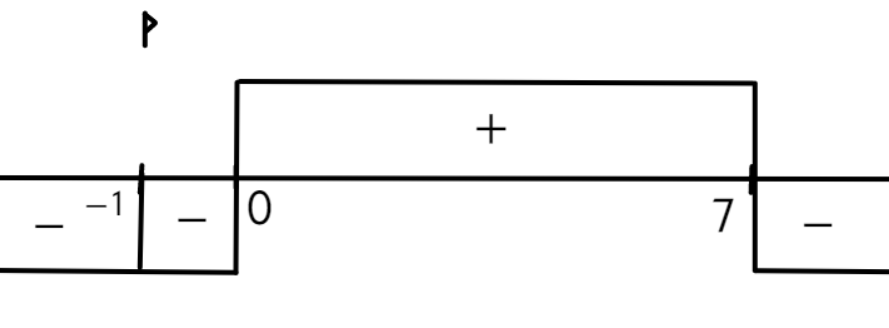
\includegraphics[scale=0.35]{int71.png}}
\end{figure}
$x\in\{-1\}\cup[0;7).$\\
72. $\cfrac{(x+1)(x-8)^4}{(x+2)^2(5-x)}\geqslant0.$ Применив метод интервалов, найдём ответ:
\begin{figure}[ht!]
\center{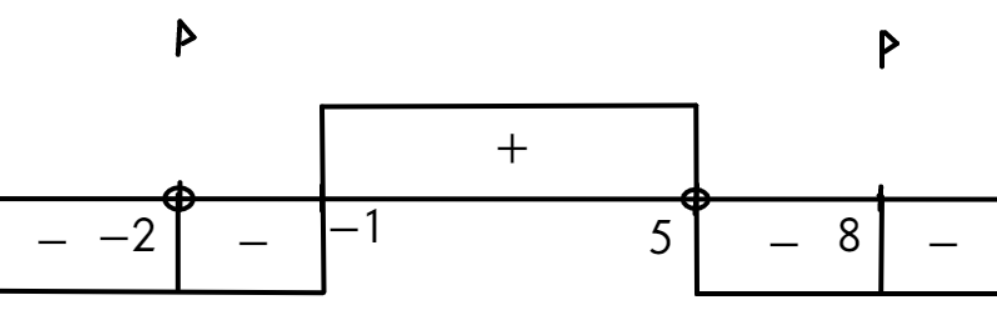
\includegraphics[scale=0.35]{int72.png}}
\end{figure}
$x\in[-1;5)\cup\{8\}.$\\
73. $\cfrac{x^2(x^2-2x+1)}{(x+7)^3(3-x)}\leqslant0\Leftrightarrow\cfrac{x^2(x-1)^2}{(x+7)^3(3-x)}\leqslant0.$\\ Применив метод интервалов, найдём ответ:
\begin{figure}[ht!]
\center{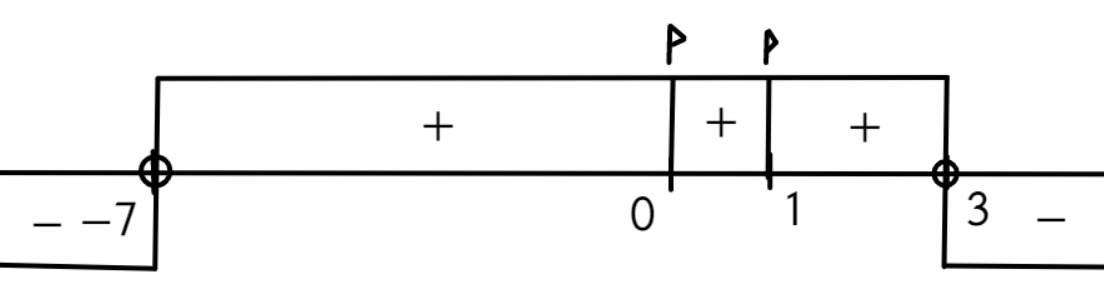
\includegraphics[scale=0.35]{int73.png}}
\end{figure}
$x\in(-\infty;-7)\cup\{0;1\}\cup(3;+\infty).$\\
74. $(2-\sqrt{5})x>2+\sqrt{5}\Leftrightarrow x<\cfrac{2+\sqrt{5}}{2-\sqrt{5}}=\cfrac{4+4\sqrt{5}+5}{4-5}=-9-4\sqrt{5}=-9-\sqrt{80}.$ Так как $9+\sqrt{80}<9+9=18,$
наибольшим целым решением неравенства является $x=-18.$\\
75. $(\sqrt{3}-2)x>\sqrt{3}+2\Leftrightarrow x<\cfrac{\sqrt{3}+2}{\sqrt{3}-2}=\cfrac{3+4\sqrt{3}+4}{3-4}=-7-4\sqrt{3}=-7-\sqrt{48}.$ Так как $7+\sqrt{48}<7+7=14,$
наибольшим целым решением неравенства является $x=-14.$\\
76. $|x-3|<6-3x\Leftrightarrow\begin{cases} x-3<6-3x,\\x-3>-6+3x.\end{cases}
\Leftrightarrow\begin{cases} x<\cfrac{9}{4},\\ x<\cfrac{3}{2}.\end{cases}\Leftrightarrow x\in\left(-\infty;\cfrac{3}{2}\right)$\\
77. $|x-4|>2x-1\Leftrightarrow\left[\begin{array}{l}x-4>2x-1,\\x-4<-2x+1.\end{array}\right.
\Leftrightarrow\left[\begin{array}{l}x<-3,\\x<\cfrac{5}{3}.\end{array}\right.\Leftrightarrow x\in\left(-\infty;\cfrac{5}{3}\right).$\\
78. $|2x-7|<x \Leftrightarrow \begin{cases} 2x-7<x,\\ 2x-7> -x\end{cases} \Leftrightarrow \begin{cases} x<7,\\ x>\cfrac{7}{3}\end{cases}
\Leftrightarrow x\in\left(\cfrac{7}{3};7\right).$\\
79. $|2x-5|<x \Leftrightarrow \begin{cases} 2x-5<x,\\ 2x-5> -x\end{cases} \Leftrightarrow \begin{cases} x<5,\\ x>\cfrac{5}{3}\end{cases}
\Leftrightarrow x\in\left(\cfrac{5}{3};5\right).$\\
80. $\cfrac{\sqrt{x+3}(2x^2+13x+15)(x^2+4x-5)(2x+3)}{x^2-1}\geqslant0 \Leftrightarrow \cfrac{\sqrt{x+3}\cdot4\left(x+\cfrac{3}{2}\right)^2(x+5)^2(x-1)}{(x-1)(x+1)}\geqslant0.$ Применив метод интервалов, найдём ответ:
\begin{figure}[ht!]
\center{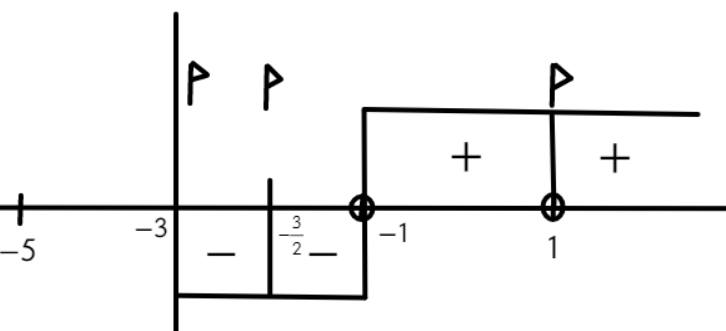
\includegraphics[scale=0.35]{int80.png}}
\end{figure}
$x\in\left\{-3;-\cfrac{3}{2}\right\}\cup(-1;1)\cup(1;+\infty).$\\
81. $\cfrac{\sqrt{x+4}(2x^2+13x+20)(x^2+4x-12)(2x+5)}{x^2-4}\geqslant0\Leftrightarrow \cfrac{\sqrt{x+4}\cdot4\left(x+\cfrac{5}{2}\right)^2(x+4)(x+6)(x-2)}{(x-2)(x+2)}\geqslant0.$ Применив метод интервалов, найдём ответ:
\begin{figure}[ht!]
\center{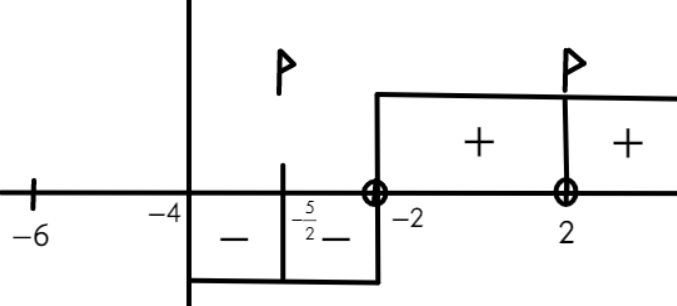
\includegraphics[scale=0.35]{int81.png}}
\end{figure}
$x\in\left\{-4;-\cfrac{5}{2}\right\}\cup(-2;2)\cup(2;+\infty).$\\
82. $\cfrac{(2x^2+7x-4)(x-3)^2}{x+6}\leqslant0\Leftrightarrow\cfrac{(2x-1)(x+4)(x-3)^2}{x+6}\leqslant0.$
Применив метод интервалов, найдём ответ:
\begin{figure}[ht!]
\center{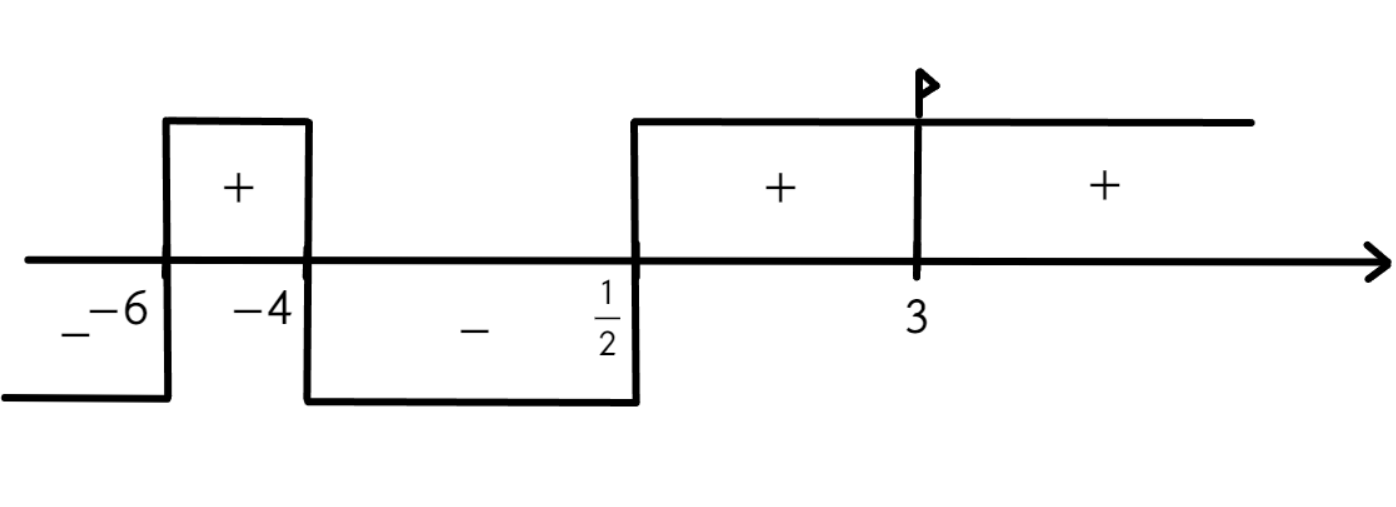
\includegraphics[scale=0.35]{int82.png}}
\end{figure}
$x\in(-\infty;-6)\cup\left[-4;\cfrac{1}{2}\right]\cup\{3\}.$\newpage\noindent
83. $\cfrac{(2x^2+5x-3)(x-4)^2}{x+5}\leqslant0\Leftrightarrow\cfrac{(2x-1)(x+3)(x-4)^2}{x+5}\leqslant0.$
Применив метод интервалов, найдём ответ:
\begin{figure}[ht!]
\center{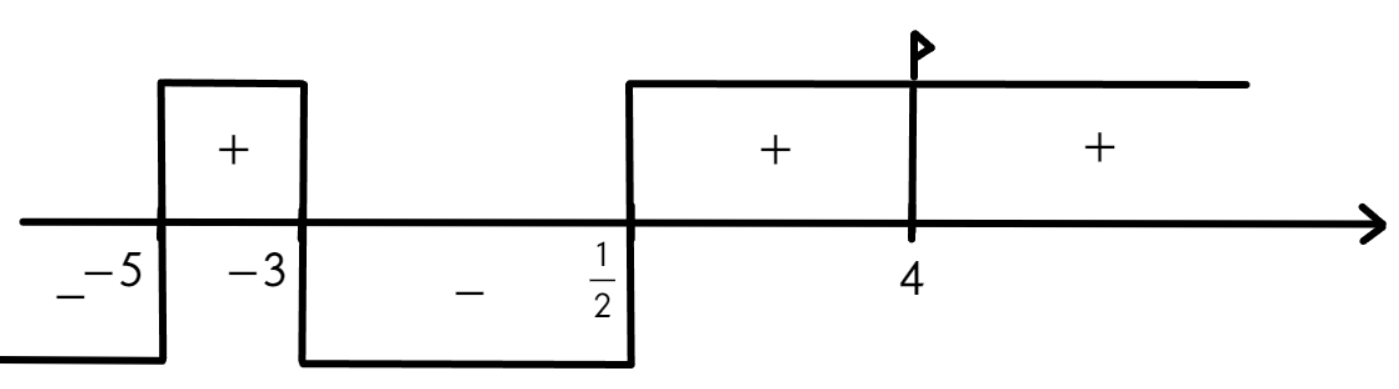
\includegraphics[scale=0.35]{int83.png}}
\end{figure}
$x\in(-\infty;-5)\cup\left[-3;\cfrac{1}{2}\right]\cup\{4\}.$\\
84. $\begin{cases} x^2+3x-4\geqslant0,\\ -x-5<0.\end{cases}\Leftrightarrow \begin{cases} (x+4)(x-1)\geqslant0,\\ x>-5.\end{cases}
\Leftrightarrow \begin{cases} x\in(-\infty;-4]\cup[1;+\infty),\\ x>-5.\end{cases}\Leftrightarrow x\in(-5;-4]\cup[1;+\infty).$\\
85. $\begin{cases} x^2+2x-3\leqslant0,\\ -x-1>0.\end{cases} \Leftrightarrow\begin{cases} (x+3)(x-1)\leqslant0,\\ x<-1.\end{cases}
\Leftrightarrow\begin{cases} x\in[-3;1],\\ x<-1.\end{cases}\Leftrightarrow x\in[-3;-1).$\\
86. $2|x-1|\geqslant 2-x\Leftrightarrow |x-1|\geqslant \cfrac{2-x}{2} \Leftrightarrow \left[\begin{array}{l} x-1\geqslant \cfrac{2-x}{2},\\
x-1\leqslant \cfrac{x-2}{2}\end{array}\right. \Leftrightarrow \left[\begin{array}{l} 2x-2-2+x\geqslant 0,\\
2x-2-x+2\leqslant 0.\end{array}\right. \Leftrightarrow \left[\begin{array}{l} x\geqslant \cfrac{4}{3},\\
x\leqslant 0.\end{array}\right. $\\$\Leftrightarrow x\in(-\infty;0]\cup\left[\cfrac{4}{3};+\infty\right).$\\
87. $2|x+1|\geqslant x+2\Leftrightarrow |x+1|\geqslant \cfrac{x+2}{2} \Leftrightarrow \left[\begin{array}{l} x+1\geqslant \cfrac{x+2}{2},\\
x+1\leqslant \cfrac{-x-2}{2}.\end{array}\right. \Leftrightarrow \left[\begin{array}{l} 2x+2-2-x\geqslant 0,\\
2x+2+x+2\leqslant 0.\end{array}\right. \Leftrightarrow \left[\begin{array}{l} x\geqslant 0,\\
x\leqslant -\cfrac{4}{3}.\end{array}\right.$\\$ \Leftrightarrow x\in\left(-\infty;-\cfrac{4}{3}\right]\cup[0;+\infty).$\\
88. $\cfrac{2|x-1|}{2-x}\geqslant1 \Leftrightarrow \cfrac{2|x-1|+x-2}{2-x}\geqslant0\Leftrightarrow
\left[\begin{array}{l}\begin{cases} \cfrac{2x-2+x-2}{2-x}\geqslant0,\\ x\geqslant 1.\end{cases}\\ \begin{cases}\cfrac{-2x+2+x-2}{2-x}\geqslant0,\\ x<1.           \end{cases}\end{array}\right.\Leftrightarrow
\left[\begin{array}{l}\begin{cases} \cfrac{3x-4}{2-x}\geqslant0,\\ x\geqslant 1.\end{cases}\\ \begin{cases}\cfrac{-x}{2-x}\geqslant0,\\ x<1.           \end{cases}\end{array}\right.\Leftrightarrow
\left[\begin{array}{l}\begin{cases} x\in\left[\cfrac{4}{3};2\right),\\ x\geqslant 1.\end{cases}\\ \begin{cases}x\in(-\infty;0]\cup(2;+\infty),\\ x<1.           \end{cases}\end{array}\right.\Leftrightarrow x\in(-\infty;0]\cup\left[\cfrac{4}{3};2\right).$\\
89. $\cfrac{2|x+1|}{x+2}\geqslant1 \Leftrightarrow \cfrac{2|x+1|-x-2}{x+2}\geqslant0\Leftrightarrow
\left[\begin{array}{l}\begin{cases} \cfrac{2x+2-x-2}{x+2}\geqslant0,\\ x\geqslant -1.\end{cases}\\ \begin{cases}\cfrac{-2x-2-x-2}{x+2}\geqslant0,\\ x<-1.           \end{cases}\end{array}\right.\Leftrightarrow
\left[\begin{array}{l}\begin{cases} \cfrac{x}{x+2}\geqslant0,\\ x\geqslant -1.\end{cases}\\ \begin{cases}\cfrac{-3x-4}{x+2}\geqslant0,\\ x<-1.           \end{cases}\end{array}\right.\Leftrightarrow
\left[\begin{array}{l}\begin{cases} x\in(-\infty;-2)\cup[0;+\infty),\\ x\geqslant -1.\end{cases}\\ \begin{cases}x\in\left(-2;-\cfrac{4}{3}\right],\\ x<-1.\end{cases}\end{array}\right.\Leftrightarrow x\in\left(-2;-\cfrac{4}{3}\right]\cup[0;+\infty).$\\
90. $\begin{cases} |x^2+2x-15|\leqslant0,\\ x^{15}-3x^{14}+2x-5>0.\end{cases}$ Модуль может не превосходить 0 только если он равен нулю, значит $x^2+2x-15=0,\
(x+5)(x-3)=0,\ x=-5$ или $x=3.$ Надо проверить, удовлетворяют ли найденные значения второму неравенству, для этого преобразуем его: $x^{15}-3x^{14}+2x-5=x^{14}(x-3)+(2x-5)>0.$ При $x=3$ левая часть равна 1, а при $x=-5$ она будет отрицательна, значит решением является только $x=3.$\\
91. $-2<\cfrac{1-x}{x}<3\Leftrightarrow \begin{cases} \cfrac{1-x}{x}+2>0,\\ \cfrac{1-x}{x}-3<0.\end{cases}\Leftrightarrow
\begin{cases} \cfrac{1+x}{x}>0,\\ \cfrac{1-4x}{x}<0.\end{cases}\Leftrightarrow \begin{cases} x\in(-\infty;-1)\cup(0;+\infty),\\ x\in (-\infty;0)\cup\left(\cfrac{1}{4};+\infty\right)\end{cases}\Leftrightarrow$\\$ x\in(-\infty;-1)\cup\left(\cfrac{1}{4};+\infty\right).$\\
92. $x\cdot|x^2-5x|\leqslant6x \Leftrightarrow \left[\begin{array}{l} \begin{cases} |x^2-5x|\leqslant6,\\ x>0.\end{cases}\\
\begin{cases} |x^2-5x|\geqslant6,\\ x<0.\end{cases}\\x=0.\end{array}\right.
\Leftrightarrow \left[\begin{array}{l} \begin{cases} x^2-5x\leqslant6,\\ x^2-5x\geqslant-6,\\ x>0.\end{cases}\\
\begin{cases} \left[\begin{array}{l}x^2-5x\geqslant6,\\ x^2-5x\leqslant-6,\end{array}\right.\\ x<0.\end{cases}\\x=0.\end{array}\right.
\Leftrightarrow$\\$ \left[\begin{array}{l} \begin{cases} (x-6)(x+1)\leqslant0,\\ (x-2)(x-3)\geqslant0,\\ x>0.\end{cases}\\
\begin{cases} \left[\begin{array}{l}(x-6)(x+1)\geqslant0,\\ (x-2)(x-3)\leqslant0,\end{array}\right.\\ x<0.\end{cases}\\x=0.\end{array}\right.$
$\Leftrightarrow\left[\begin{array}{l} \begin{cases} x\in[-1;6],\\ x\in(-\infty;2]\cup[3;+\infty),\\ x>0.\end{cases}\\
\begin{cases} \left[\begin{array}{l}x\in(-\infty;-1]\cup[6;+\infty),\\ x\in[2;3],\end{array}\right.\\ x<0.\end{cases}\\x=0.\end{array}\right.
\Leftrightarrow\left[\begin{array}{l} x\in(0;2]\cup[3;6],\\
x\in(-\infty;-1],\\x=0.\end{array}\right.\Leftrightarrow $\\$x \in (-\infty;-1]\cup[0;2]\cup[3;6].$\\
93. $\cfrac{3}{5x-1}+\cfrac{4}{3x+1}\geqslant1\Leftrightarrow\cfrac{9x+3+20x-4-15x^2-5x+3x+1}{(5x-1)(3x+1)}\geqslant 0\Leftrightarrow
\cfrac{3x(9-5x)}{(5x-1)(3x+1)}\geqslant 0.$ Применив метод интервалов, найдём ответ:
\begin{figure}[ht!]
\center{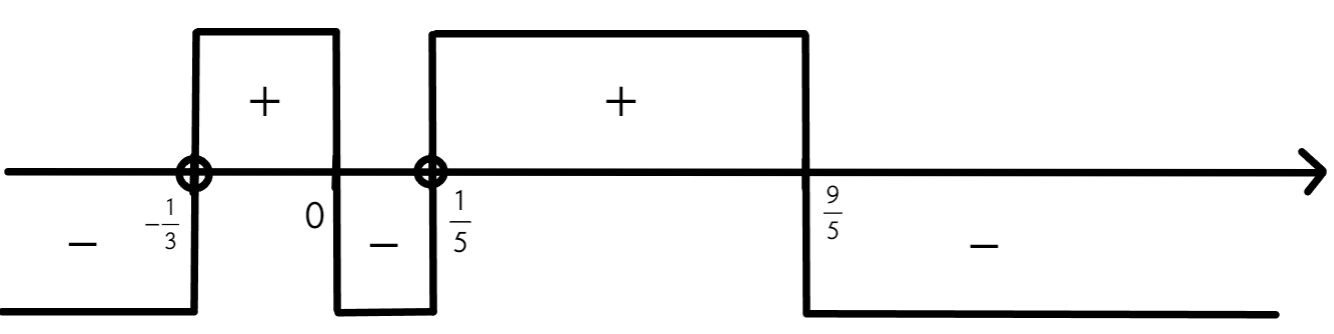
\includegraphics[scale=0.35]{int93.png}}
\end{figure}
$x\in\left(-\cfrac{1}{3};0\right]\cup\left(\cfrac{1}{5};\cfrac{9}{5}\right].$\newpage\noindent
94. $\cfrac{5}{2x+1}+\cfrac{2}{7x-1}\leqslant3\Leftrightarrow\cfrac{35x-5+4x+2-42x^2+6x-21x+3}{(2x+1)(7x-1)}\leqslant 0\Leftrightarrow
\cfrac{6x(4-7x)}{(2x+1)(7x-1)}\leqslant 0.$ Применив метод интервалов, найдём ответ:
\begin{figure}[ht!]
\center{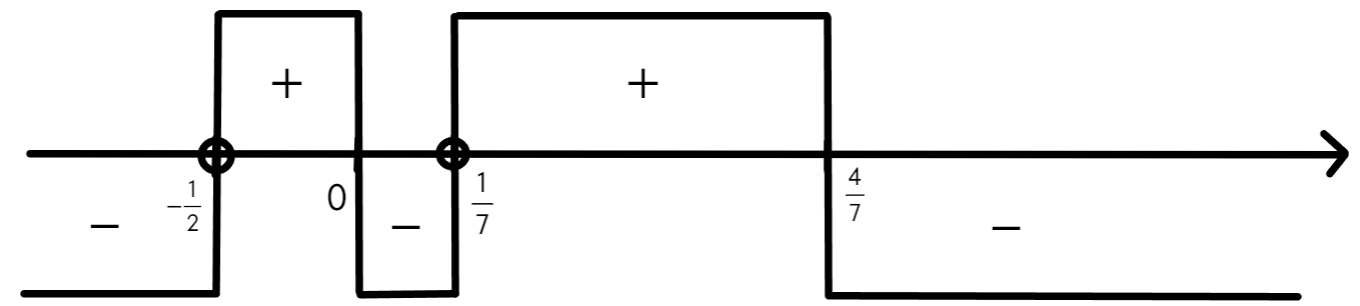
\includegraphics[scale=0.35]{int94.png}}
\end{figure}
$x\in\left(-\infty;-\cfrac{1}{2}\right)\cup\left[0;\cfrac{1}{7}\right)\cup\left(\cfrac{4}{7};+\infty\right).$\\
95. $\cfrac{(x^2-3x+2)(1-x)}{x-3}\geqslant0\Leftrightarrow\cfrac{(x-2)(x-1)(1-x)}{x-3}\geqslant0\Leftrightarrow\cfrac{(x-2)(x-1)^2}{x-3}\leqslant0.$ Применив метод интервалов, найдём ответ:
\begin{figure}[ht!]
\center{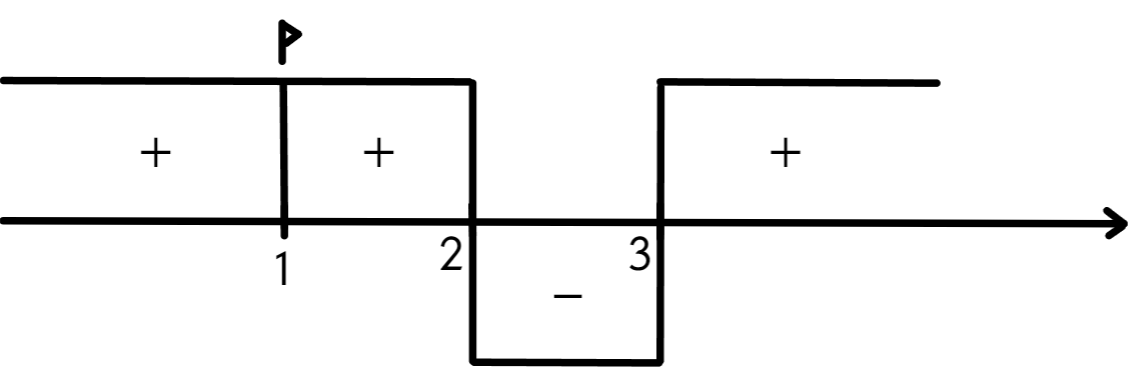
\includegraphics[scale=0.35]{int95.png}}
\end{figure}
$x\in\{1\}\cup[2;3).$\\
96. $\cfrac{3x^3}{x-5}\geqslant\cfrac{-2x^2}{5-x}\Leftrightarrow\cfrac{3x^3}{x-5}\geqslant\cfrac{2x^2}{x-5}\Leftrightarrow
\cfrac{3x^3-2x^2}{x-5}\geqslant0\Leftrightarrow\cfrac{x^2(3x-2)}{x-5}\geqslant0.$ Применив метод интервалов, найдём ответ: $x\in\left(-\infty;\cfrac{2}{3}\right]
\cup(5;+\infty).$
\begin{figure}[ht!]
\center{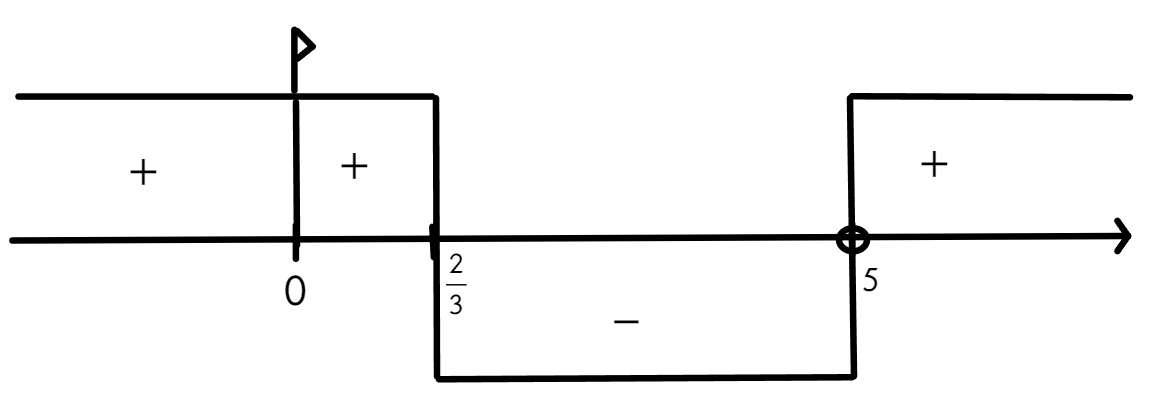
\includegraphics[scale=0.35]{ner30-1.png}}
\end{figure}\\
97. $|x+2|+|x-2|\leqslant2x\Leftrightarrow\left[\begin{array}{l}\begin{cases}-x-2-x+2\leqslant2x,\\ x\leqslant-2\end{cases}\\
\begin{cases}x+2-x+2\leqslant2x,\\ -2\leqslant x \leqslant 2\end{cases}\\
\begin{cases}x+2+x-2\leqslant2x,\\ 2\leqslant x \end{cases}
\end{array}\right.\Leftrightarrow\left[\begin{array}{l}\begin{cases}-4x\leqslant0,\\ x\leqslant-2\end{cases}\\
\begin{cases}4\leqslant2x,\\ -2\leqslant x \leqslant 2\end{cases}\\
\begin{cases}0\leqslant0,\\ 2\leqslant x \end{cases}
\end{array}\right.\Leftrightarrow x\in[2;+\infty).$\newpage\noindent
98. $\cfrac{(x-7)\sqrt{x+5}}{x^6-16x^2}\geqslant0\Leftrightarrow
\cfrac{(x-7)\sqrt{x+5}}{x^2(x-2)(x+2)(x^2+4)}\geqslant0.$ Применив метод интервалов, найдём ответ: $x\in\{-5\}\cup(-2;0)\cup(0;2)\cup[7;+\infty).$
\begin{figure}[ht!]
\center{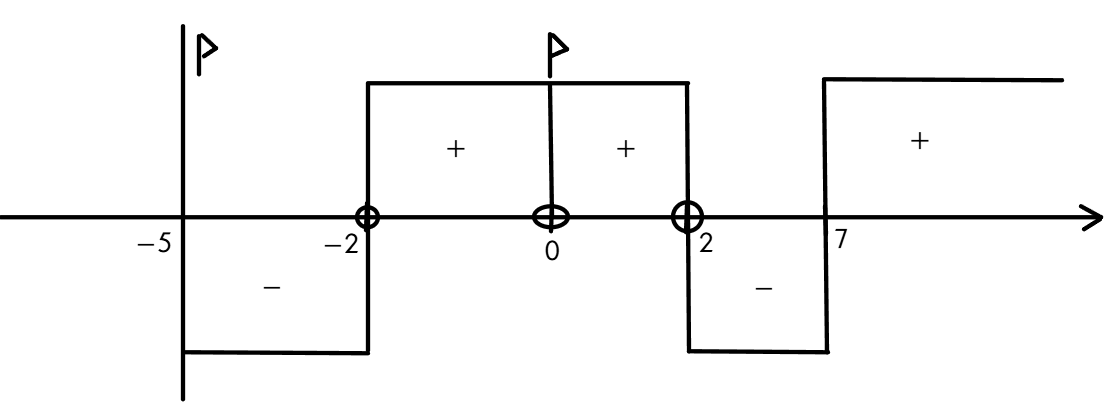
\includegraphics[scale=0.35]{int97.png}}
\end{figure}\\
99. $\cfrac{(x-5)\sqrt{x+7}}{x^6-81x^2}\geqslant0\Leftrightarrow
\cfrac{(x-5)\sqrt{x+7}}{x^2(x-3)(x+3)(x^2+9)}\geqslant0.$ Применив метод интервалов, найдём ответ: $x\in\{-7\}\cup(-3;0)\cup(0;3)\cup[5;+\infty).$
\begin{figure}[ht!]
\center{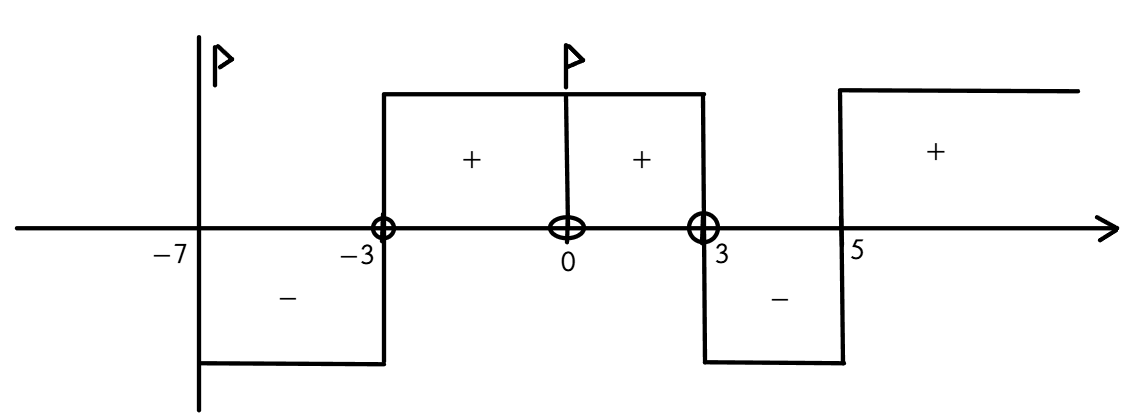
\includegraphics[scale=0.35]{int96.png}}
\end{figure}\\
100. $\cfrac{x^3-9x^2+20x}{x-4}\leqslant0\Leftrightarrow \cfrac{x(x^2-9x+20)}{x-4}\leqslant0\Leftrightarrow\cfrac{x(x-4)(x-5)}{x-4}\leqslant0.$ Применив метод интервалов, найдём ответ: $x\in[0;4)\cup(4;5].$
\begin{figure}[ht!]
\center{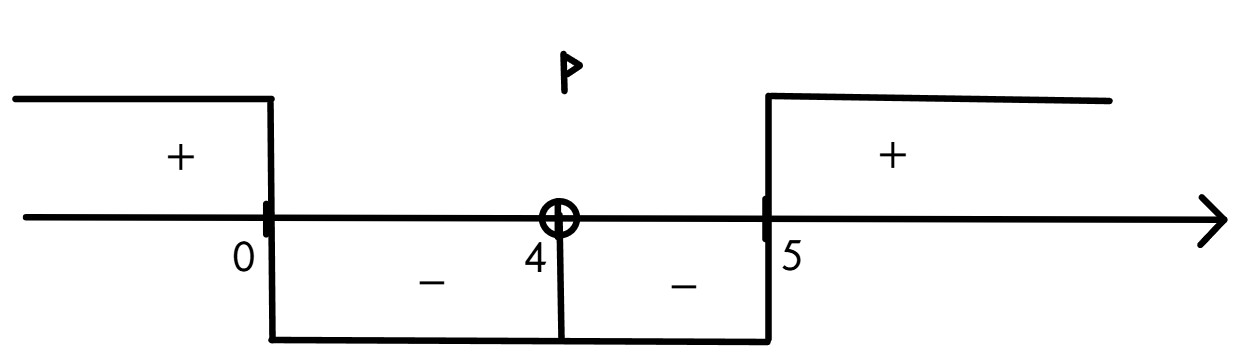
\includegraphics[scale=0.35]{int85.png}}
\end{figure}\\
101. $\cfrac{x^3-8x^2+15x}{x-3}\leqslant0\Leftrightarrow \cfrac{x(x^2-8x+15)}{x-3}\leqslant0\Leftrightarrow\cfrac{x(x-3)(x-5)}{x-3}\leqslant0.$ Применив метод интервалов, найдём ответ: $x\in[0;3)\cup(3;5].$
\begin{figure}[ht!]
\center{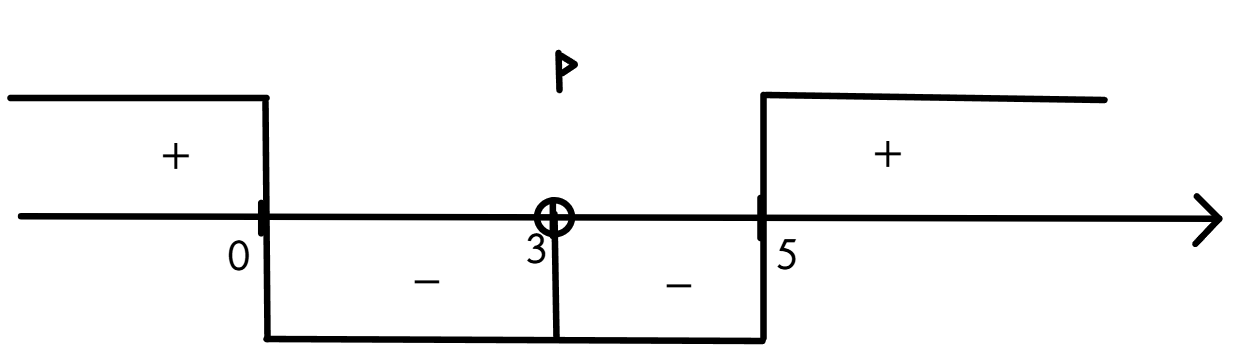
\includegraphics[scale=0.35]{int84.png}}
\end{figure}
\newpage
